\section{Resultados}

\subsection{Gr\'aficos de funciones (ejemplos del ejecuci\'on correcta)}

Para testear el correcto funcionamiento del int\'erprete probamos a plotear las 
funciones provistas por la catedra en los archivos \texttt{hard\_spiral},
\texttt{hard\_mosaico} y \texttt{hard\_koch}. 

Los resultados fueron los siguientes:

\begin{figure}[!ht]
        \centering
        \begin{subfigure}[b]{0.32\textwidth}
                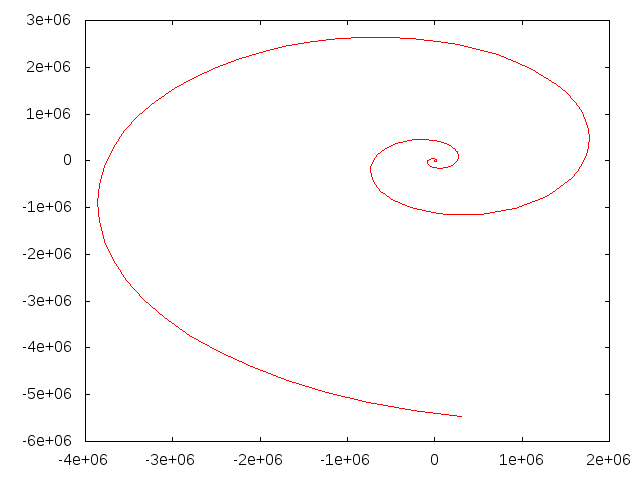
\includegraphics[width=\textwidth]{imgResu/spiral.png}
                \caption{Puntos obtenidos para el archivo \texttt{hard\_spiral}}
        \end{subfigure}%
        ~ %add desired spacing between images, e. g. ~, \quad, \qquad, \hfill etc.
          %(or a blank line to force the subfigure onto a new line)
        \begin{subfigure}[b]{0.32\textwidth}
                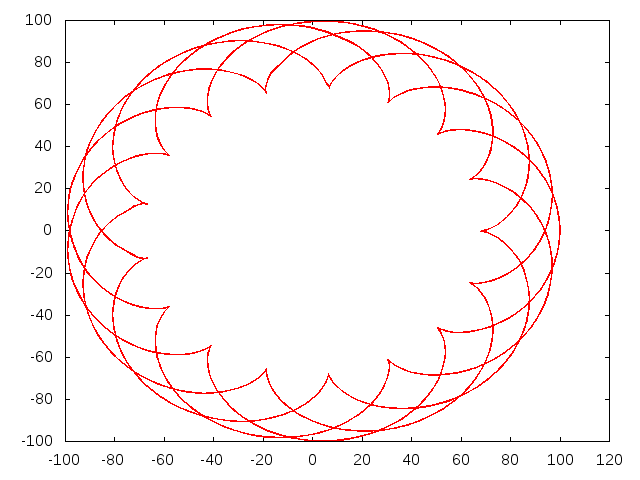
\includegraphics[width=\textwidth]{imgResu/mosaico.png}
                \caption{Puntos obtenidos para el archivo \texttt{hard\_mosaico}}
        \end{subfigure}
        ~ %add desired spacing between images, e. g. ~, \quad, \qquad, \hfill etc.
          %(or a blank line to force the subfigure onto a new line)
        \begin{subfigure}[b]{0.32\textwidth}
                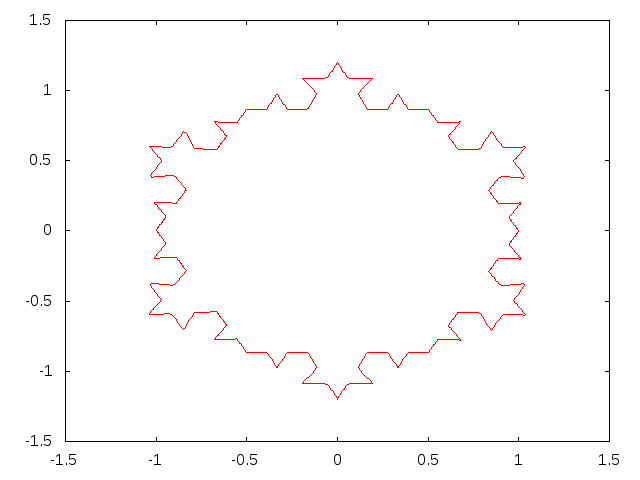
\includegraphics[width=\textwidth]{imgResu/koch.png}
                \caption{Puntos obtenidos para el archivo \texttt{hard\_koch}}
        \end{subfigure}
        \caption{Gr\'aficos obtenidos para las funciones hard: spiral, mosaico y koch}
\end{figure}

M\'as all\'a de que los gr\'aficos parezcan correctos, chequeamos que la diferencia
entre los puntos obtenidos, con los provistos por la c\'atedra, fuera peque\~na.
Vimos que la diferencia rondaba $1{\times}10^{-13}$, con lo cual nos consideramos
satisfechos.

Para realizar este test utilizamos el comando:
\begin{verbatim}
paste archivo1.dat archivo2.dat | awk '{print $3 - $1, $4 - $2}'
\end{verbatim}
que compara, respectivamente, las dos columnas de dos archivos distintos.

\subsubsection{Ambig\"uedades}
La \'unica ambiguedad que encontramos en la especificaci\'on no-formal del
enunciado, es el caso del $if then else$. En particular, en el caso de tener
varios anidados, donde no se use una llave para delimitar el bloque del
\textit{then}. El problema aqu\'i reside en que no es inmediato determinar
a qu\'e \textit{if} corresponde un \textit{else} dado.

Investigando en internet (y recordando un ejercicio de la gu\'ia) llegamos
a la conclusi\'on de que la soluci\'on usual, es la de asociar el \textit{else}
al \textit{if} m\'as cercano (a la izquierda obviamente), como ya fue detallado
previamente.

\subsection{Errores (ejemplos de ejecuci\'on incorrecta)}

Para testear que las herramientas detectaran errores en los archivos 
utilizamos los test brindados por la c\'atedra.

Los resultados en los archivos uno, dos y cinco fueron: 
\subsubsection{Archivo uno}
\begin{verbatim}
Interpreter: 
9:9: Error de parseo. Justo antes de:

(x,10) for x=-1..0.5..5*(pi+(1
\end{verbatim}

\subsubsection{Archivo dos}
\begin{verbatim}
Interpreter: 
4:9: Error de parseo. Justo antes de:

id(x)) for x=-10..0.5..5

/*
\end{verbatim}

\subsubsection{Archivo cinco}
\begin{verbatim}
Interpreter: 
3:14: Error de parseo. Justo antes de:

 {
        return a
    }
\end{verbatim}

Mientras que para el tercer y cuarto archivo fueron:

\subsubsection{Archivo tres}
\begin{verbatim}
Interpreter: 
Runtime error: funcion id no declarada
\end{verbatim}

\subsubsection{Archivo cuatro}
\begin{verbatim}
Interpreter: 
Runtime error: cantidad incorrecta de parametros en constpi
\end{verbatim}
